\documentclass[11pt]{article}
%%%%%%%%%%%%%%%%
% Packages
%%%%%%%%%%%%%%%%

\usepackage[top=1cm,bottom=1.1cm,left=1.25cm,right= 1.25cm]{geometry}
\usepackage[parfill]{parskip}
\usepackage{graphicx, fontspec, xcolor,multicol, enumitem, setspace, amsmath, changepage}
\DeclareGraphicsRule{.tif}{png}{.png}{`convert #1 `dirname #1`/`basename #1 .tif`.png}

%%%%%%%%%%%%%%%%
% User defined colors
%%%%%%%%%%%%%%%%

% Pantone 2015 Fall colors
% http://iwork3.us/2015/02/18/pantone-2015-fall-fashion-report/
% update each semester or year

\xdefinecolor{custom_blue}{rgb}{0, 0.32, 0.48} % FROM SPRING 2016 COLOR PREVIEW
\xdefinecolor{custom_darkBlue}{rgb}{0.20, 0.20, 0.39} % Reflecting Pond  
\xdefinecolor{custom_orange}{rgb}{0.96, 0.57, 0.42} % Cadmium Orange
\xdefinecolor{custom_green}{rgb}{0, 0.47, 0.52} % Biscay Bay
\xdefinecolor{custom_red}{rgb}{0.58, 0.32, 0.32} % Marsala

\xdefinecolor{custom_lightGray}{rgb}{0.78, 0.80, 0.80} % Glacier Gray
\xdefinecolor{custom_darkGray}{rgb}{0.35, 0.39, 0.43} % Stormy Weather

%%%%%%%%%%%%%%%%
% Color text commands
%%%%%%%%%%%%%%%%

%orange
\newcommand{\orange}[1]{\textit{\textcolor{custom_orange}{#1}}}

% yellow
\newcommand{\yellow}[1]{\textit{\textcolor{yellow}{#1}}}

% blue
\newcommand{\blue}[1]{\textit{\textcolor{blue}{#1}}}

% green
\newcommand{\green}[1]{\textit{\textcolor{custom_green}{#1}}}

% red
\newcommand{\red}[1]{\textit{\textcolor{custom_red}{#1}}}

%%%%%%%%%%%%%%%%
% Coloring titles, links, etc.
%%%%%%%%%%%%%%%%

\usepackage{titlesec}
\titleformat{\section}
{\color{custom_blue}\normalfont\Large\bfseries}
{\color{custom_blue}\thesection}{1em}{}
\titleformat{\subsection}
{\color{custom_blue}\normalfont}
{\color{custom_blue}\thesubsection}{1em}{}

\newcommand{\ttl}[1]{ \textsc{{\LARGE \textbf{{\color{custom_blue} #1} } }}}

\newcommand{\tl}[1]{ \textsc{{\large \textbf{{\color{custom_blue} #1} } }}}

\usepackage[colorlinks=false,pdfborder={0 0 0},urlcolor= custom_orange,colorlinks=true,linkcolor= custom_orange, citecolor= custom_orange,backref=true]{hyperref}

%%%%%%%%%%%%%%%%
% Instructions box
%%%%%%%%%%%%%%%%

\newcommand{\inst}[1]{
\colorbox{custom_blue!20!white!50}{\parbox{\textwidth}{
	\vskip10pt
	\leftskip10pt \rightskip10pt
	#1
	\vskip10pt
}}
\vskip10pt
}

%%%%%%%%%%%
% App Ex number    %
%%%%%%%%%%%

% DON'T FORGET TO UPDATE

\newcommand{\appno}[1]
{4.4}

%%%%%%%%%%%%%%
% Turn on/off solutions       %
%%%%%%%%%%%%%%

% Off
\newcommand{\soln}[2]{$\:$\\ \vspace{#1}}{}

%%% On
%\newcommand{\soln}[2]{\textit{\textcolor{custom_red}{#2}}}{}

%%%%%%%%%%%%%%%%
% Document
%%%%%%%%%%%%%%%%

\begin{document}
\fontspec[Ligatures=TeX]{Helvetica Neue Light}

Dr. \c{C}etinkaya-Rundel \hfill Sta 101: Data Analysis and Statistical Inference \\
Duke University - Department of Statistical Science \hfill \\

\ttl{Application exercise \appno{}: \\
ANOVA}

\inst{$\:$ \\
Team name: \rule{10cm}{0.5pt} \\
$\:$ \\
Lab section: $\qquad$ 8:30 $\qquad$ 10:05 $\qquad$ 11:45 $\qquad$ 1:25 $\qquad$ 3:05 \\
$\:$ \\
Write your responses in the spaces provided below. WRITE LEGIBLY and SHOW ALL WORK! 
Only one submission per team is required. One team will be randomly selected and their 
responses will be discussed and graded. Concise and coherent are best!}

%%%%%%%%%%%%%%%%%%%%%%%%%%%%%%%%%%%%

\section*{Teacher evaluations}

Many college courses conclude by giving students the opportunity to evaluate the course and the instructor 
anonymously. In this application exercise we evaluate whether the teaching evaluations for instructors vary 
by their rank: teaching, tenure track, and tenured. Note that the instructors are evaluated on a 1-5 scale (1-low, 5-high). 
The data come from ``Beauty in the classroom: instructors' pulchritude and putative pedagogical productivity'' 
(Hamermesh and Parker, 2005) found that instructors who are viewed to be better looking receive higher 
instructional ratings.

{\scriptsize Daniel S. Hamermesh, Amy Parker, Beauty in the classroom: instructors' pulchritude 
and putative pedagogical productivity, \textit{Economics of Education Review}, Volume 24, Issue 4, August 2005, 
Pages 369-376, ISSN 0272-7757, 10.1016/j.econedurev.2004.07.013. \\
\href{http://www.sciencedirect.com/science/article/pii/S0272775704001165}{http://www.sciencedirect.com/science/article/pii/S0272775704001165}.} 

{\small
\begin{center}
\begin{tabular}{l | c | c | c | c | c | c | c | c}
		& Min. & 1st Qu. & Median  &  Mean & 3rd Qu. &   Max. & Std. Dev. & n \\
\hline
teaching	&  3.300 &  3.900  & 4.400&   4.284 &  4.700&   5.000 	& 0.5 & 102 \\
tenure track	& 2.300 &  3.700 &  4.350  & 4.155 &  4.600  & 4.900 & 0.56 & 108 \\
tenured 	&   2.400   & 3.800 &  4.200  & 4.139  & 4.600 &  5.000  & 0.55 & 253
\end{tabular}
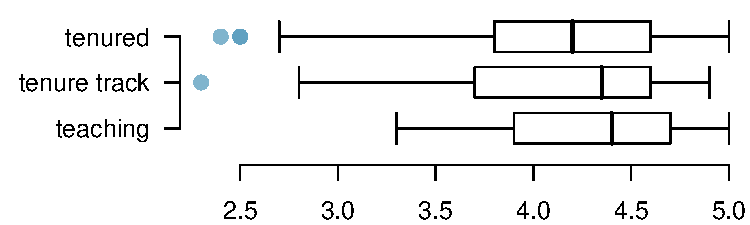
\includegraphics[width=0.5\textwidth]{figures/evals_rank}
\end{center}
}

%

\begin{enumerate}

\item What is the response variable in the ANOVA? \_\_\_\_\_\_\_\_\_\_\_\_\_\_ \soln{0cm}{Eval score}

\item What is the explanatory variable in the ANOVA? \_\_\_\_\_\_\_\_\_\_\_\_\_\_ \soln{0cm}{Rank}

\item State the hypotheses for evaluating whether the average evaluation score varies by rank.

\soln{5cm}{
$H_0$: Average eval score does not vary by rank. \\
$H_A$: Average eval score varies by rank, at least two means are different. 
}

\vfill

\pagebreak

\item Check the conditions for evaluating these hypotheses.

\soln{3cm}{
\begin{enumerate}
\item Independent observations: Random sampling + each group less than 10\% of its respective population
\item Normality: Distributions of each group not normal (left skewed) but n is large so not a huge deal
\item Constant variance: Variability across groups somewhat consistent
\end{enumerate}
}

\item Below is a partial ANOVA table. Fill in the blanks. \textit{Hint:} Not all blanks in the table need to be filled, 
you need to decide which blanks need to be filled.

\begin{center}
\renewcommand{\arraystretch}{1.5}
\begin{tabular}{l | p{1.5cm} | p{2cm} | p{2cm} | p{2cm} | p{2cm} }
  \hline
 			& Df 		& Sum Sq 	& Mean Sq 	& F 		 & p-value \\ 
  \hline
rank 			&  		& 1.59 		&  			& 	 	&  \\ 
\hline
Residuals 		& 	 	& 	 		& 	 		& 		&  \\ 
\hline
Total			&		& 136.66		&			&		&
\end{tabular}
\end{center}

\soln{2cm}
{
\begin{itemize}
\item Df: $df_G = 3 - 1 = 2$, $df_T = (102 + 108 + 253) - 1 = 462$, $df_E = 462 - 2 = 460$ \\
\item SS: $SS_E = 136.66 - 1.59 = 135.07$ \\
\item MS: $MS_G = 1.59 / 2 = 0.795$, $MS_E = 135.07 / 462 = 0.29$ \\
\item F = 0.795 / 0.29 = 2.74 \\
\item p-value = \texttt{pf(2.74, df1 = 2, df2 = 462, lower.tail = FALSE)} = 0.065
\end{itemize}
}

\item Determine the conclusion of the hypothesis test at $\alpha = 0.10$.

\soln{3cm}
{
Reject $H_0$. At least one pair of means are different from each other.
}

\item Explain what the sum of squares associated with rank (also called $SS_{group}$) and sum of squares 
associated with the residuals (also called $SS_{error}$) and the total sum of squares also called $SS_{total}$) mean. You are not being 
asked to calculate these numbers, only to explain what they mean in context of the data.

\soln{5cm}
{
$SS_G$: Variability between groups \\
$SS_E$: Variability within groups \\
$SS_T$: Total variability in evaluation scores
}

\pagebreak

\item What percent of variability in evaluation scores is explained by the rank of professors?

\soln{3cm}
{$SS_G / SS_T = 1.59 / 136.66 = 0.0116 \rightarrow 1.16\%$}

\item We want to determine which means are different from each other. What significance level should we use 
for these tests and why?

\soln{3cm}
{
$\alpha^\star = 0.10 / 3 = 0.033$
}

\item Conduct at least one of these tests (or all, time permitting) and determine which means are different.
\textit{Hint:} You're doing a post-hoc pairwise tests, how are $SE$ and $df$ defined?

\soln{3cm}
{Do t tests where variance is MSE and df is $df_E$ for all tests}

\end{enumerate}

%%%%%%%%%%%%%%%%%%%%%%%%%%%%%%%%%%%%

\end{document}